% This is a LaTeX thesis template for Adam Mickiewicz University.
% to be used with Rmarkdown
% This template was produced by Jakub Nowosad
% Version: 16 February 2020

% Inspired by:
% This is a LaTeX thesis template for Monash University.
% to be used with Rmarkdown
% This template was produced by Rob Hyndman
% Version: 6 September 2016

\documentclass{amuthesis}
\usepackage{polski}
\renewcommand{\figurename}{Rycina} % Redefine default figure caption %
\renewcommand{\tablename}{Tabela} % Redefine default table caption %
%%%%%%%%%%%%%%%%%%%%%%%%%%%%%%%%%%%%%%%%%%%%%%%%%%%%%%%%%%%%%%%
% Add any LaTeX packages and other preamble here if required
%%%%%%%%%%%%%%%%%%%%%%%%%%%%%%%%%%%%%%%%%%%%%%%%%%%%%%%%%%%%%%%
\usepackage{booktabs,tabularx} % Allows kableExtra to work %
\usepackage{indentfirst} % Adds indent in the first paragraph %

\author{Maria Król}
\title{Porównanie technik przestrzennej wizualizacji wyników wyborów w Polsce}
\def\titleeng{2020 presidential election results in Poland - comparsion of spatial visualisation techniques}
\def\degreetitle{Praca inżynierska}
\def\major{Geoinformacja}
\def\albumid{431977}
\def\thesisyear{2021}
% Add subject and keywords below
\hypersetup{
     %pdfsubject={The Subject},
     %pdfkeywords={Some Keywords},
     pdfauthor={Maria Król},
     pdftitle={Porównanie technik przestrzennej wizualizacji wyników wyborów w Polsce},
     pdfproducer={Bookdown with LaTeX}
}

\bibliography{thesis,packages}

\begin{document}

\pagenumbering{arabic}

\titlepage

\hypertarget{streszczenie}{%
\section*{Streszczenie}\label{streszczenie}}
\addcontentsline{toc}{section}{Streszczenie}

Streszczenie powinno przedstawiać skrótowo główny problem pracy i jego rozwiązanie.
Możliwa struktura streszczenia to: (1) 1-3 zdania wstępu do problemu (czym się zajmujemy, dlaczego jest to ważne, jakie są problemy/luki do wypełnienia), (2) 1 zdanie opisujące cel pracy, (3) 1-3 zdania przedstawiające użyte materiały (dane) i metody (techniki, narzędzia), (4) 1-3 zdania obrazujące główne wyniki pracy, (5) 1-2 zdania podsumowujące; możliwe jest też określenie dalszych kroków/planów.

Słowa kluczowe: (4-6 słów/zwrotów opisujących treść pracy, które nie wystąpiły w tytule)

\hypertarget{abstract}{%
\section*{Abstract}\label{abstract}}
\addcontentsline{toc}{section}{Abstract}

The abstract must be consistent with the above text.

Keywords: (as stated before)

\newpage

\setstretch{1.2}\sf\tighttoc\doublespacing

\hypertarget{wprowadzenie}{%
\chapter{Wprowadzenie}\label{wprowadzenie}}

Wybory są jednym z podstawowych narzędzi współczesnych demokracji.
Demokracja pośrednia, znana również jako przedstawicielska, jest dominującą formą demokracji na świecie, funkcjonuje ona również w Polsce.
Encyklopedia PWN (2020) definiuje wybory jako \textit{„sposób powoływania obywateli do pełnienia funkcji publicznych w organach państwowych, a także w organach samorządowych, partii politycznych i in. organizacji społecznych, przez głosowanie na wysuniętych kandydatów lub ich listy.”}

\begin{figure}[!H]

{\centering \includegraphics[width=400px,]{figures/ryc11} 

}

\caption{Mapa wyborów prezydenckich w Stanach Zjednoczonych w 1880 roku. Źródło: http://www.mappingthenation.com/blog/the-nations-first-electoral-map/}\label{fig:ryc11}
\end{figure}

Historia map wyborczych sięga ponad 200 lat, kiedy w 1869 roku odbyły się wybory parlamentarne w Paryżu.
Mapa pokazuje obrazuje zmieniający się nastrój polityczny w stolicy, który doprowadził do zamieszek wewnętrznych, a ostatecznie do wielkiej wojny międzynarodowej i upadku Drugiego Cesarstwa Francuskiego \autocite{cartographia2008}.
Najstarsza znana mapa wyborów prezydenckich pochodzi jednak z Atlasu Statystycznego Stanów Zjednoczonych opublikowanego w 1883 roku i przedstawia wyniki na poziomie stanów i hrabstw z wyborów prezydenckich w 1880 roku \autocite{schulten2013}.
Mapa nie tylko pokazuje, która partia wygrała w każdym z hrabstw, ale także ukazuje przewagę partii za pomocą cieniowania gradientowego (Ryc. \ref{fig:ryc11}).

Postęp w technikach kartograficznych nabrał tempa wraz z rozwojem drukarstwa oraz możliwością tworzenia niestandardowych grafik do gazet \autocite{kongres2013}.
Pozwoliło to na spopularyzowanie mapy jako formy reprezentacji danych wyborczych oraz w konsekwencji, rozwój technik tworzenia map (Ryc. \ref{fig:ryc12}-\ref{fig:ryc13}).

Pomimo swojej długiej historii, mapy wyborcze stały się popularne dopiero w ciągu ostatnich 30 lat.
W połączeniu z rozwojem technologii mapy stały się jednymi z najbardziej efektywnych sposobów uwieczniania informacji o charakterze przestrzennym, w tym danych wyborczych.
Pozwalają one nam szybko i łatwo przeanalizować informacje.
Główną zaletą wizualizacji przestrzennych jest możliwość odnoszenia ich do wybranych lokalizacji lub jednostek administracyjnych.
Możliwość iteracji pozwala na tworzeniu wielu wizualizacji za pomocą tych samych danych.

\begin{figure}[h]

{\centering \includegraphics[width=300px]{figures/ryc12} 

}

\caption{Mapa wyborów prezydenckich w Stanach Zjednoczonych w 1896 roku. Źródło: https://mode.com/blog/presenting-data-election-maps}\label{fig:ryc12}
\end{figure}

\begin{figure}[h]

{\centering \includegraphics[width=200px]{figures/ryc13} 

}

\caption{Mapa wyborów parlamentarnych w Wielkiej Brytanii w 1895 roku. Źródło: http://www.ericson.net/content/2010/11/first-nyt-election-map/}\label{fig:ryc13}
\end{figure}

Jedną z rozwijających się kierunków badań w zakresie kartografii jest wizualizacja.
Gałąź ta powstała w latach 90. XX wieku wskutek rozwoju oraz upowszechnienia się technologii komputerowych.
W porównaniu do kartografii, wizualizacja jest elementem procesu poznawczej analizy danych przestrzennych, a jej celem jest odkrywanie prawidłowości i informacji w danych o charakterze przestrzennym. \autocite{maceachren1994}.

W Polsce wybory są regulowane przez ustawę z dnia 5 stycznia 2011 r. - \href{https://pkw.gov.pl/uploaded_files/1598525869_kodeks-wyborczy-2020-lipiec.pdf}{Kodeks wyborczy}.
Ustawa ta weszła w życie 1 sierpnia 2011 roku i zawiera przepisy dotyczące m.in. przeprowadzania wyborów prezydenckich.
Znajdują się w niej również przepisy o warunkach ważności wyborów i przepisy karne za wykroczenia i niektóre przestępstwa popełnione przeciwko wyborom.
Za organizację i przebieg wyborów odpowiada w Polsce Państwowa Komisja Wyborcza (PKW) z Krajowym Biurem Wyborczym (KBW), które jest jej organem wykonawczym.
Zadaniem Państwowej Komisji Wyborczej jest również gromadzenie oraz udostępnianie informacji wyborczych, w tym wyników wyborów z poziomu obwodów wyborczych oraz jednostek administracyjnych.

Powszechne, w pełni demokratyczne wybory prezydenckie III Rzeczypospolitej odbyły się po raz pierwszy 25 listopada 1990 roku.
Wybory prezydenckie odbywają się na zarządzenie Marszałka Sejmu, a kadencja trwa 5 lat.
Ostatnie wybory na prezydenta RP zostały przeprowadzone 28 czerwca 2020 roku \autocite{marszalek2020}.

W przypadku Polski historyczne mapy wyborcze znajdują się m.in. w Atlasie Rzeczypospolitej Polskiej, gdzie przedstawione są wybory prezydenckie z 1990 (Ryc. \ref{fig:ryc14}) i 1995 roku (Ryc. \ref{fig:ryc15}). W obu przypadkach przedstawione są wyłącznie kartogramy skokowe, pola odniesienia ograniczono do województw oraz gmin.

\begin{figure}[h]

{\centering 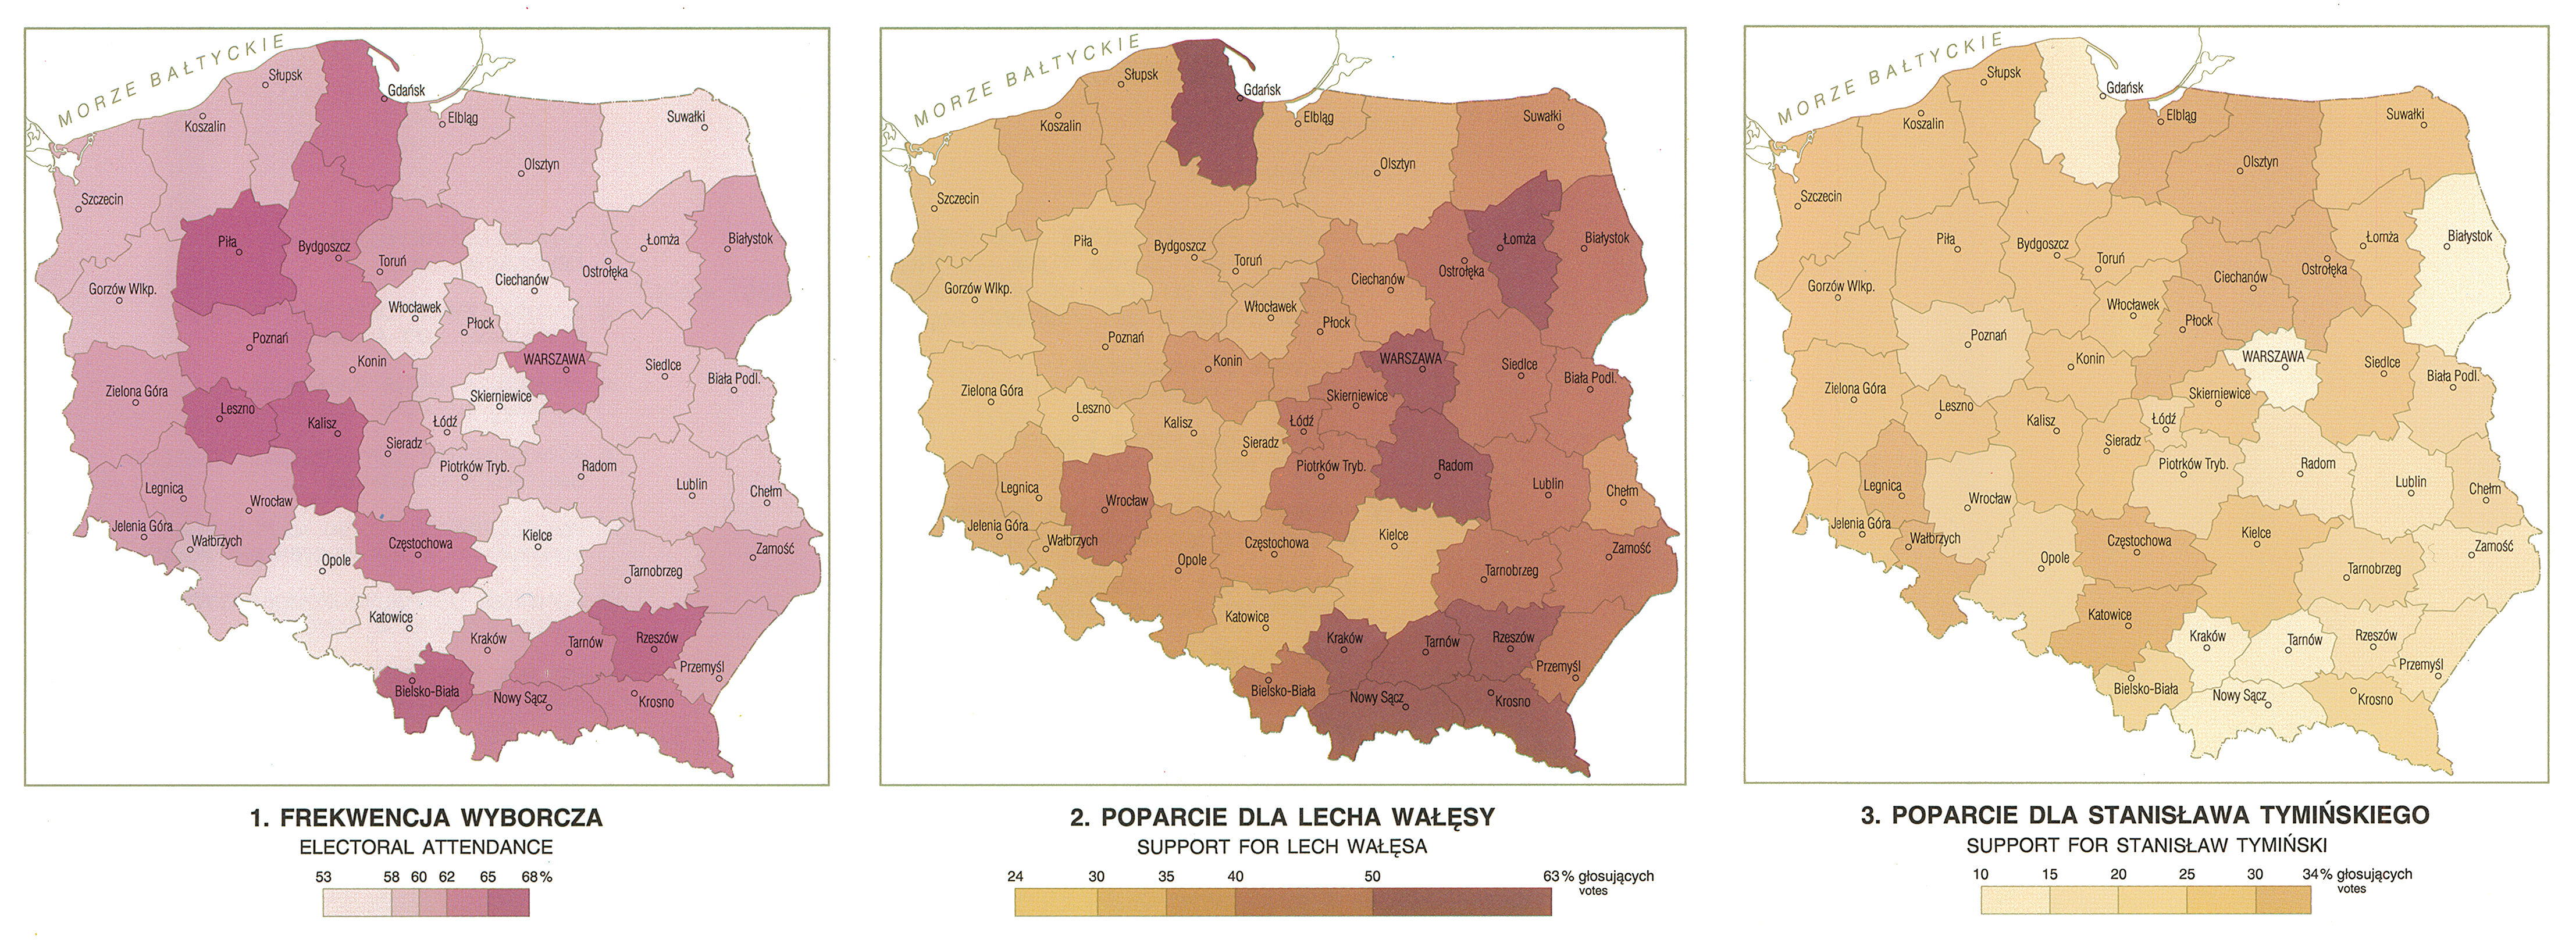
\includegraphics[width=400px]{figures/ryc14} 

}

\caption{Mapa wyborów prezydenckich w Polsce w 1990 roku. Źródło: Atlas Rzeczypospolitej Polskiej}\label{fig:ryc14}
\end{figure}

\begin{figure}[h]

{\centering 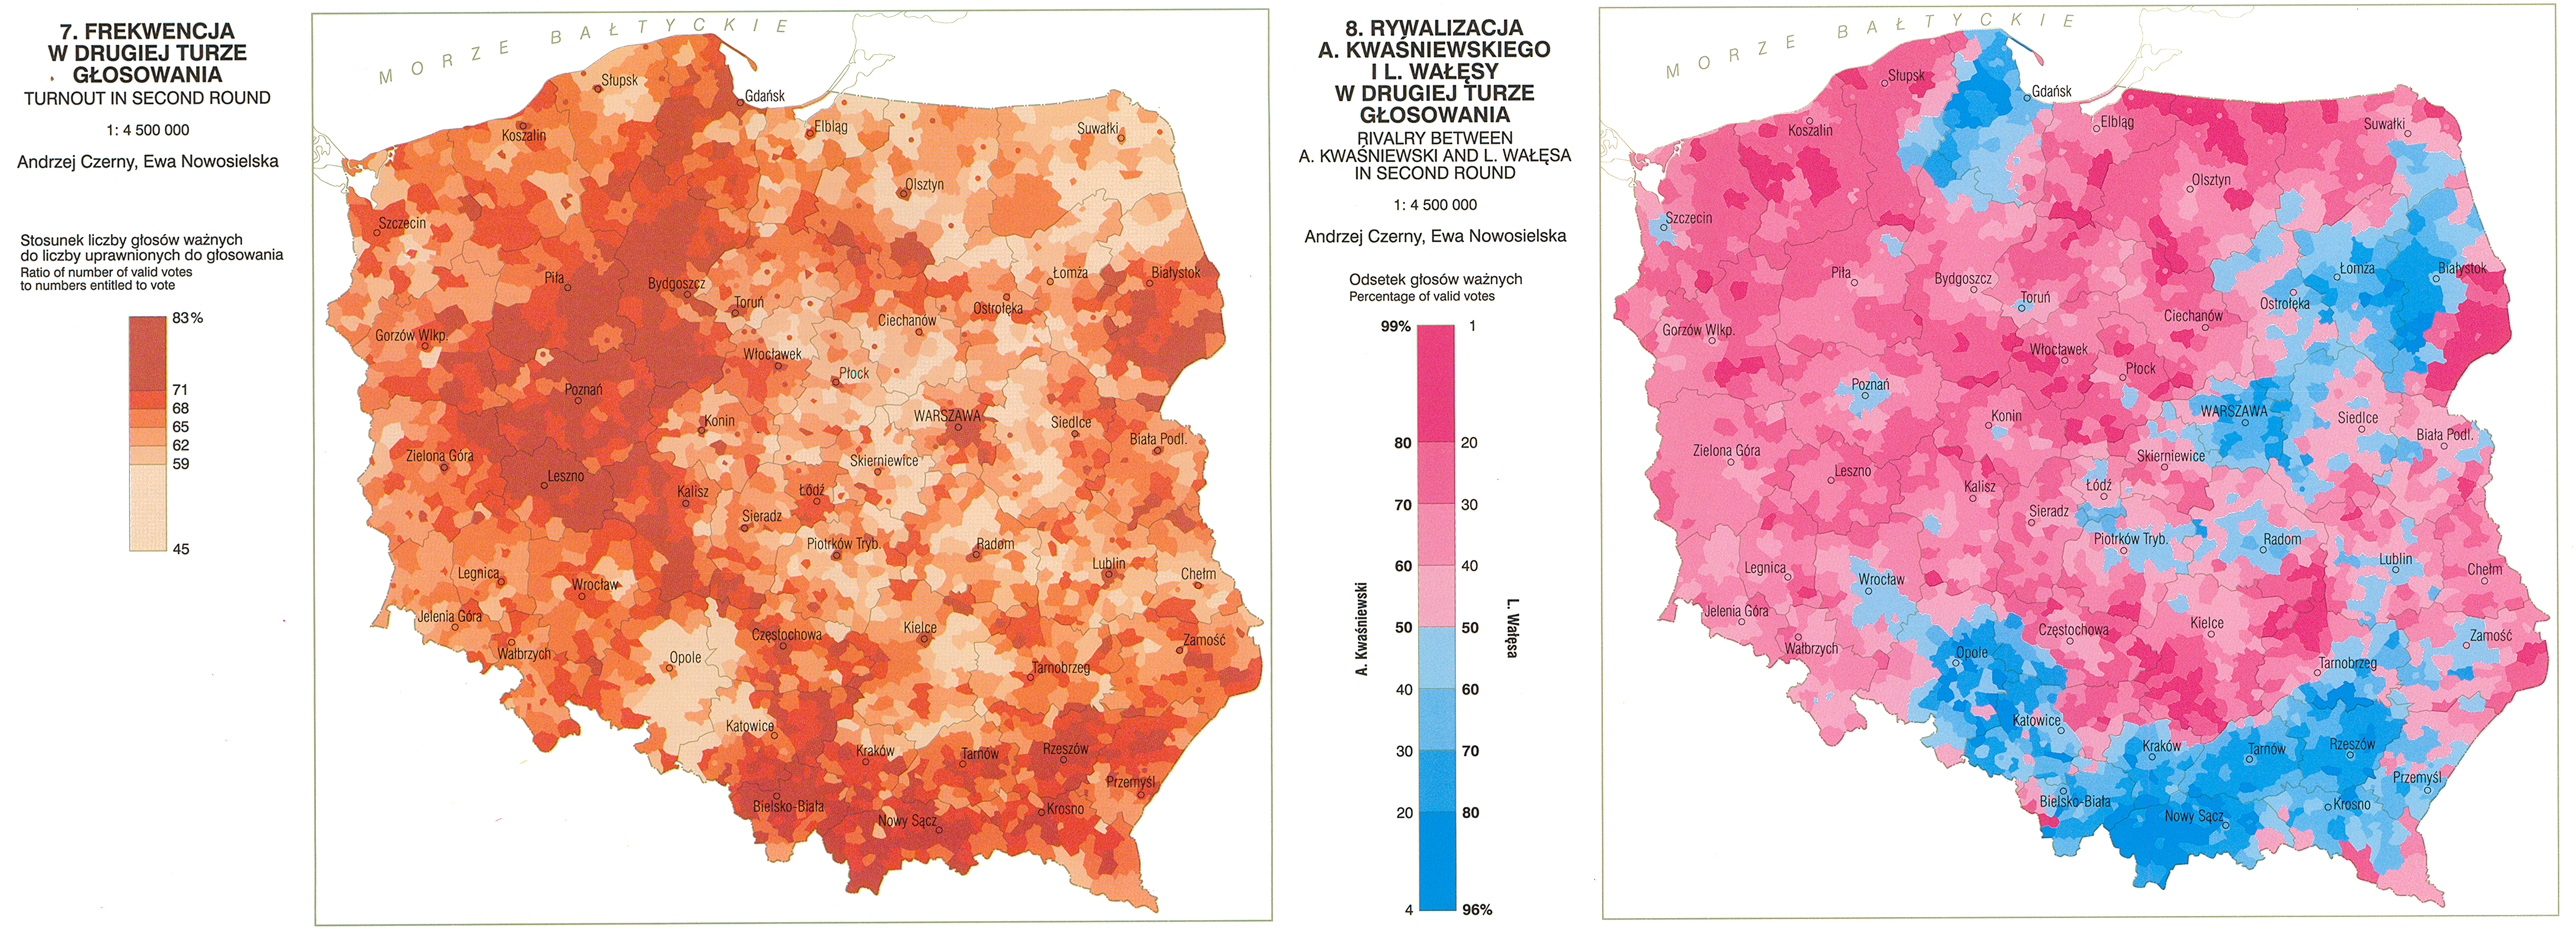
\includegraphics[width=400px]{figures/ryc15} 

}

\caption{Mapa wyborów prezydenckich w Polsce w 1995 roku. Źródło: Atlas Rzeczypospolitej Polskiej}\label{fig:ryc15}
\end{figure}

Jak wspomniano wyżej, wizualizacja map wyborczych w Polsce ogranicza się w znacznej części do kartogramów skokowych.
Istnieją inne formy wizualizacji, które przykładają mniejszą wagę do powierzchni i pozwalają na dokładniejsze przedstawienie wartości.
Są to, m.in., kartogramy geometryczne oraz anamorfozy (kartogramy odwrócone).
Niska popularność tych form jest związana z przyzwyczajeniem społeczeństwa do analizowania map opartych o jednostki administracyjne jak powiaty lub województwa.
Trudność potrafią sprawić również zniekształcenia związane z anamorfozą, w skrajnych przypadkach powierzchnia jednostki odniesienia może być nie do rozpoznania.
Do prawidłowej interpretacji powyżej wspomnianych dwóch rodzajów map niezbędna jest również wiedza o rozmiarach i rozmieszczeniu jednostek.

Celem pracy jest porównanie różnych technik wizualizacji na przykładzie wyborów prezydenckich w 2020 roku w Polsce.
Nastąpiło to poprzez przygotowanie map używając metod kartogramu właściwego, kartogramu ciągłego, kartogramu geometrycznego, anamorfozy ciągłej, nieciągłej i kartodiagramu Dorlinga oraz oceniono pod względem stopnia ich czytelności.
Podjęto również próbę porównania właściwości rozpatrywanych technik oraz określenia zakresu ich zastosowania; szukano odpowiedzi na pytanie o to, jaką i na ile dokładną informację można uzyskać na podstawie każdej z technik.
W tym celu zostały zebrane oraz opracowane dane z Państwowej Komisji Wyborczej, które następnie posłużyły do stworzenia wizualizacji - do tego użyto dwa pakiety z języka R: \emph{cartogram} \autocite{r-cartogram} oraz \emph{geogrid} \autocite{r-geogrid}.
Opracowane zostały dwie wersje ankiety mające na celu ocenę stopnia trudności interpretacji wizualizacji.
Ankiety została przeprowadzone z udziałem studentów trzeciego oraz czwartego roku studiów na Wydziale Nauk Geograficznych i Geologicznych UAM, a w oparciu o jej wyniki przeprowadzono analizę czytelności każdej z technik wizualizacji.

\hypertarget{lit}{%
\chapter{Przegląd literatury}\label{lit}}

Placeholder

\hypertarget{kartogramy1}{%
\section{Kartogramy właściwe oraz ciągłe}\label{kartogramy1}}

\hypertarget{kartogramy-geometryczne}{%
\section{Kartogramy geometryczne}\label{kartogramy-geometryczne}}

\hypertarget{kartogramy-eumorficzne}{%
\section{Kartogramy eumorficzne}\label{kartogramy-eumorficzne}}

\hypertarget{metody}{%
\chapter{Metody}\label{metody}}

Placeholder

\hypertarget{dane}{%
\section{Dane}\label{dane}}

\hypertarget{biblioteki}{%
\section{Biblioteki języka R}\label{biblioteki}}

\hypertarget{wizualizacje}{%
\chapter{Wizualizacje}\label{wizualizacje}}

Placeholder

\hypertarget{kartogramwlasciwy}{%
\section{Kartogram właściwy}\label{kartogramwlasciwy}}

\hypertarget{kartogramyciagle}{%
\section{Kartogramy ciągłe}\label{kartogramyciagle}}

\hypertarget{kartogramygeometryczne}{%
\section{Kartogramy geometryczne}\label{kartogramygeometryczne}}

\hypertarget{anamorfozaciagla}{%
\section{Anamorfoza ciągła}\label{anamorfozaciagla}}

\hypertarget{anamorfozanieciagla}{%
\section{Anamorfoza nieciągła}\label{anamorfozanieciagla}}

\hypertarget{kartodiagramdorlinga}{%
\section{Kartodiagram Dorlinga}\label{kartodiagramdorlinga}}

\hypertarget{ankieta}{%
\chapter{Ankieta}\label{ankieta}}

Placeholder

\hypertarget{ankietyintro}{%
\section{Ankiety dotyczące map wyborczych}\label{ankietyintro}}

\hypertarget{pyt1}{%
\subsection{Pytanie pierwsze}\label{pyt1}}

\hypertarget{pyt2}{%
\subsection{Pytanie drugie}\label{pyt2}}

\hypertarget{pyt3}{%
\subsection{Pytanie trzecie}\label{pyt3}}

\hypertarget{pyt4}{%
\subsection{Pytanie czwarte}\label{pyt4}}

\hypertarget{pyt5}{%
\subsection{Pytanie piąte}\label{pyt5}}

\hypertarget{pyt6}{%
\subsection{Pytanie szóste}\label{pyt6}}

\hypertarget{pyt7}{%
\subsection{Pytanie siódme}\label{pyt7}}

\hypertarget{wnioski}{%
\section{Wnioski}\label{wnioski}}

\hypertarget{podsumowanie}{%
\chapter{Podsumowanie}\label{podsumowanie}}

Placeholder

\printbibliography[heading=bibintoc, title=Bibliografia]

\end{document}
